\documentclass[11pt]{article}

\input{../../../fimacros.tex}

\setheadings{MTH 288 --- Linear Algebra --- Syllabus, Fall 2016}

\setlength\parindent{0pt}

\begin{document}

\sffamily

\begin{center}

{\large Cleveland State University --- Department of Mathematics}

\bigskip
{\Large \textbf{Syllabus for MTH 288}}

\medskip 
{\Large \textbf{Linear Algebra}}

\medskip
Fall 2016: August 29 -- December 15
\end{center}

\section{Instructor Information}
\begin{tabular}{ll}
\textbf{Instructor}: & Dr. L. Felipe Martins.\\
\textbf{Office}: &  RT1533\\
\textbf{E-mail}: &  \href{mailto:l.martins@csuohio.edu}{l.martins@csuohio.edu}\\
\textbf{Phone}: & 216--687--4683 \\
\textbf{Office Hours}: & MWF 10:30 AM -- 12:00 PM or by appointment.\\
%\textbf{}: &  \\
\end{tabular}

\section{Meeting Place}

Regular classroom: BU 109 (MF)

Computer Lab: RT 1501 (W)

\section{Textbook}

\emph{Linear Algebra}, by David Cherney, Tom Denton and Andrew Waldron. The book can be downloaded for free from \url{https://www.math.ucdavis.edu/~linear/linear-guest.pdf}

\section{Course Description}
Linear algebra is one of the basic core disciplines in mathematics, and is central to many subjects in pure and applied mathematics, such as multivariable calculus, ordinary and partial differential equations, differential geometry, algebraic geometry and functional analysis. It also has direct applications in diverse areas in science and engineering, including optimization, mathematical modeling, probability and statistics, mechanics, electrical circuits, error-correcting codes, and many others. Linear algebra one of the major unifying ideas in mathematics, and good grasp of it is essential to anyone doing advanced work in mathematics, science and engineering.

Modern linear algebra is, of necessity, a computational discipline, since today's problems are too large to be solved by hand. In this course, we will learn to use Numpy and Scilab, which are extensive libraries for numeric calculations, based on the computer language Python. The software is open-source, is available in our computer labs, and can be freely downloaded and installed in your own computer. The course software can be downloaded from \url{https://www.continuum.io/downloads}. We will use the Python 3.5 version.

The class will meet every Wednesday in the department's computer lab, RT 1501.

The following sections of the text will be covered:

\begin{itemize}
\item[1.1] What Are Vectors?
\item[1.2] What Are Linear Functions?
\item[1.3] What is a Matrix?
\item[2.1] Gaussian Elimination
\item[2.3] Elementary Row Operations
\item[2.5] Solution Sets for Systems of Linear Equations
\item[4.1] Addition and Scalar Multiplication in $\R^n$
\item[4.2] Hyperplanes
\item[4.3] Directions and Magnitudes
\item[4.4] Vectors,Lists and Functions
\item[5.1] Examples of Vector Spaces
\item[5.2] Other Fields
\item[6.1] The Consequence of Linearity
\item[6.2] Linear Functions on Hyperplanes
\item[6.3] Linear Differential Operators
\item[6.4] Bases (Take1)
\item[7.1] Linear Transformations and Matrices
\item[7.3] Properties of Matrices
\item[7.5] Inverse Matrix
\item[8.1] The Determinant Formula
\item[8.2] Elementary Matrices and Determinants
\item[8.4] Properties of the Determinant
\item[9.1] Subspaces
\item[9.2] Building Subspaces
\item[10.1] Showing Linear Dependence
\item[10.2] Showing Linear Independence
\item[10.3] From Dependent to Independent
\item[11.1] Bases in $\R^n$
\item[11.2] Matrix of a Linear Transformation (Redux)
\item[12.1] Invariant Directions
\item[12.2] The Eigenvalue?Eigenvector Equation
\item[12.3] Eigenspaces
\item[13.1] Diagonalizability
\item[13.2] Change of Basis
\item[13.3] Changing to a Basis of Eigenvectors	
\item[14.1] Properties of the Standard Basis
\item[14.2] Orthogonal and Orthonormal Bases
\item[14.3] Relating Orthonormal Bases
\item[15.1] Diagonalizing Symmetric Matrices
\item[16.1] Range
\item[16.2] Image
\item[16.3] Summary
\item[17.1] Projection Matrices
\item[17.2] Singular Value Decomposition
\end{itemize}

\section{Assessment}

\subsection{Homework (10\%)}
Online homework is accessible through the link:

\begin{center}
\url{http://webworks2.csuohio.edu/webwork2/CSU_MTH288_Fall2016/}
\end{center}

To log in, use your 7-digit CSU ID in both the  \emph{Username} and \emph{Password} fields. Please change your password after the first login.

\emph{Being unable to access the electronic homework is not an acceptable excuse to obtain a homework deadline extension}. Students should do homework on a daily basis, as content is presented in class. Remember the old saying, ``\emph{A problem a day keeps poor grades away}''.

Understanding how to use the software to solve linear algebra problems is an integral part of the course, and students are expected to be able to use the course software to help in the solution of problems, both in the homework and in tests. 

In this course, we use open-source tools for computational mathematics, available in the department's computer labs. The software is free, and can be downloaded from:

\begin{center}
\url{https://www.continuum.io/downloads}
\end{center}

\emph{\textbf{Note}: Download the 3.5 version of Python}.

\subsection{Tests (60\%)} In-class tests account for 60\% of the overall score. There will be two tests, with closed books and notes. Tests are taken in the computer lab, and require use of the course software.

Tests will be held on the following dates:
\begin{center}
\begin{tabular}{|c|c|l|}\hline
\textbf{Test}   & \textbf{Date} & \textbf{Topics}\\\hline\hline
1 & October 12  & 1.1, 1.2, 1.3, 2.1, 2.3, 2.5, 4.1, 4.2, 4.3, \\
  &             & 4.4, 5.1, 5.2, 6.1, 6.2, 6.3, 7.1, 7.3, 7.5, \\
  &             & 8.1, 8.2, 8.4 \\\hline
2 & November 30 & 9.1, 9.2, 10.1, 10.2, 10.3, 11.1, 11.2, 12.1, \\
  &             & 12.2, 12.3, 13.1, 13.2, 13.3, 14.1, 14.2, \\
  &             & 14.3, 15.1, 16.1, 16.2, 16.3 \\ \hline
\end{tabular}
\end{center}

\textbf{Make-up Policy}: Make-ups can be given, at the instructor's discretion, for missed tests that have a valid reason, such as a medical emergency involving the student or immediate family members. 

In all cases, \emph{the student must present documentation justifying the absence}, and provide contact information for the person providing the documentation. The following reasons will \emph{not} be accepted as excuses for taking a make-up:
\begin{itemize}
\item Travel, unless it is related to a medical emergency.
\item Work commitments. If you have a work-related schedule conflict, you must arrange with your employer to receive a dispensation.
\item Medical conditions for which you cannot provide documentation. If you didn't visit a doctor office or other medical facility, you can obtain a note from the nurse's office at the university.
\item Having another test in the same day.
\item Not being able to prepare for the test.
\end{itemize}

Unless an extended absence is justified, make-ups have to be taken within three days of the test date, excluding days the university is closed. If you know in advance that you will be unavailable at a particular date, please contact your instructor as soon as possible.


\subsection{Final exam (30\%)} The final is a comprehensive test with closed books and notes, taking place on the following date:

\begin{center}
{\Large Monday, December 12, 12:30 to 2:30}

\emph{Note: The final is in the computer lab}
\end{center}

\subsection{Grade assignment} Percent scores are rounded up to the next integer, and grades are assigned according to the following table:

\begin{center}
  \begin{tabular}{c|cl}
    \hline
    \textbf{Percent score} & \multicolumn{2}{c}{\textbf{Grade}}\\
    \hline
    95 to 100	&& \ \texttt{A}\\
    90 to 94 	&& \ \texttt{A-}\\
    86 to 89 	&& \ \texttt{B+}\\
    83 to 85	&& \ \texttt{B}  \\
    80 to 82	&& \ \texttt{B-} \\
    75 to 59	&& \ \texttt{C+} \\
    70 to 74	&& \ \texttt{C}  \\
    60 to 69	&& \ \texttt{D}  \\
    59 and under && \ \texttt{F}
  \end{tabular}
\end{center}

\section{General Policies}

\subsection {Grade reporting and disputes} All student scores will be posted in Blackboard
as course work and tests are done. Students are responsible for checking their own progress, and
reporting to the instructor any discrepancies as soon as they are noticed. It is also strongly suggested
that you retain all graded work from the course until the end of the semester and grades are posted.
This way if a dispute arises concerning a recorded grade and the actual grade, we have the documentation
needed to rectify the situation. Additionally, graded works make for excellent study materials for upcoming
exams.  

\subsection{Class Conduct}
Class attendance and participation is essential for success in this course. Please come to class prepared,
and take an active role in class discussions and activities.

Please bring a graphing calculator to each class.  Cell phones should be turned off or placed on vibrate.
Text messaging during class is not appropriate and grounds for removal from class.  During computer lab 
sessions, checking email and surfing the web is inappropriate when the instructor is talking and again 
grounds for removal from the class.  Other serious disruptions are grounds for removal as well.

\subsection{Withdrawals}
Withdrawing from the course may put you in violation
of the federally mandated standards for academic progress (SAP) that you must maintain to be eligible for 
financial aid.  Read the link on the course website for information about the implications of withdrawing 
from the course for your financial aid or visit Campus 411.

\subsection{Scholastic Dishonesty}
Cheating and/or plagiarism will not be tolerated. ``Cheating'' includes copying or receiving help from
another student on quizzes, tests or exams, as well as allowing another student to copy from your work. 
Merely copying another student's homework, or allowing someone else to do your homework for you, is also 
considered cheating. If cheating occurs in a quiz or unit test, the student will receive a grade of 0 for 
that component of the course. If cheating occurs in the final exam, the student will receive a grade of F in 
the course. Any cheating activity may be reported for further action.  Information regarding the official
CSU policy regarding cheating and plagiarism can be found in the  CSU Code of Student Conduct at 
\href{http://www.csuohio.edu/studentlife/StudentCodeOfConduct.pdf}{http://www.csuohio.edu/studentlife/StudentCodeOfConduct.pdf}

\subsection{Disabilities Statement} 
Educational access is the provision of classroom accommodations, auxiliary aids and services to ensure 
equal educational opportunities for all students regardless of their disability. Any student who feels 
he or she may need an accommodation based on the impact of a disability should contact the Office of 
Disability Services at (216) 687-2015. The Office is located in MC 147. Accommodations need to be 
requested in advance and will not be granted retroactively.

\subsection{Disclaimer}
The instructor, reserves the right to modify these procedures 
as the course progresses, and to change the assignment schedule from the outline given. Any changes will 
be announced in class with adequate advance notice. You are responsible for being aware of any changes 
discussed in class and/or in the BBLearn course site. This includes exam days, homework due dates and changes 
in policy.

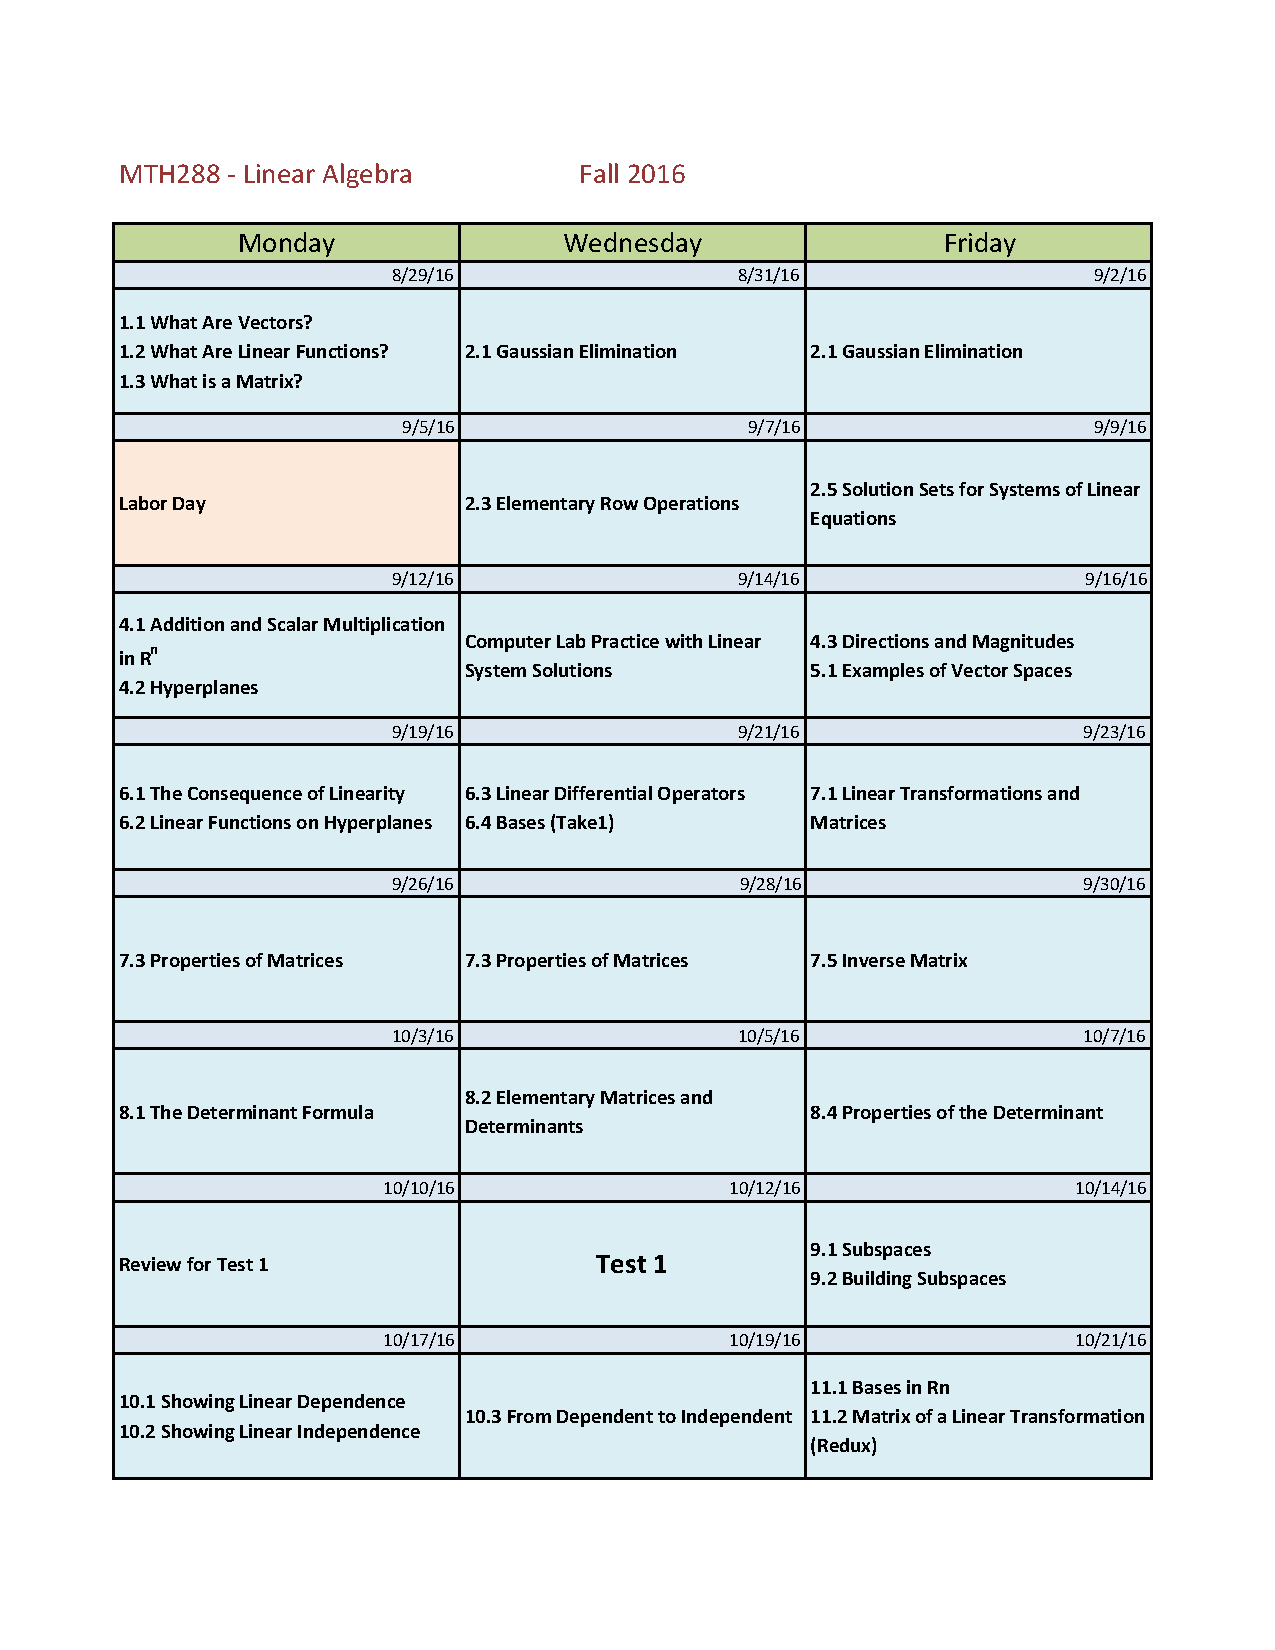
\includepdf[pages={-}]{schedule-mth288-fall2016.pdf}

\end{document}

